\documentclass[fontsize=11pt]{article}
\usepackage{amsmath}
\usepackage[utf8]{inputenc}
\usepackage[margin=0.75in]{geometry}
\usepackage{graphicx}

\title{CSC111 Project: Computing Optimal Flight Paths}
\author{JUAN MARTIN G. DE AGÜERO}
\date{\today}

\begin{document}
\maketitle

\begin{SCfigure}
    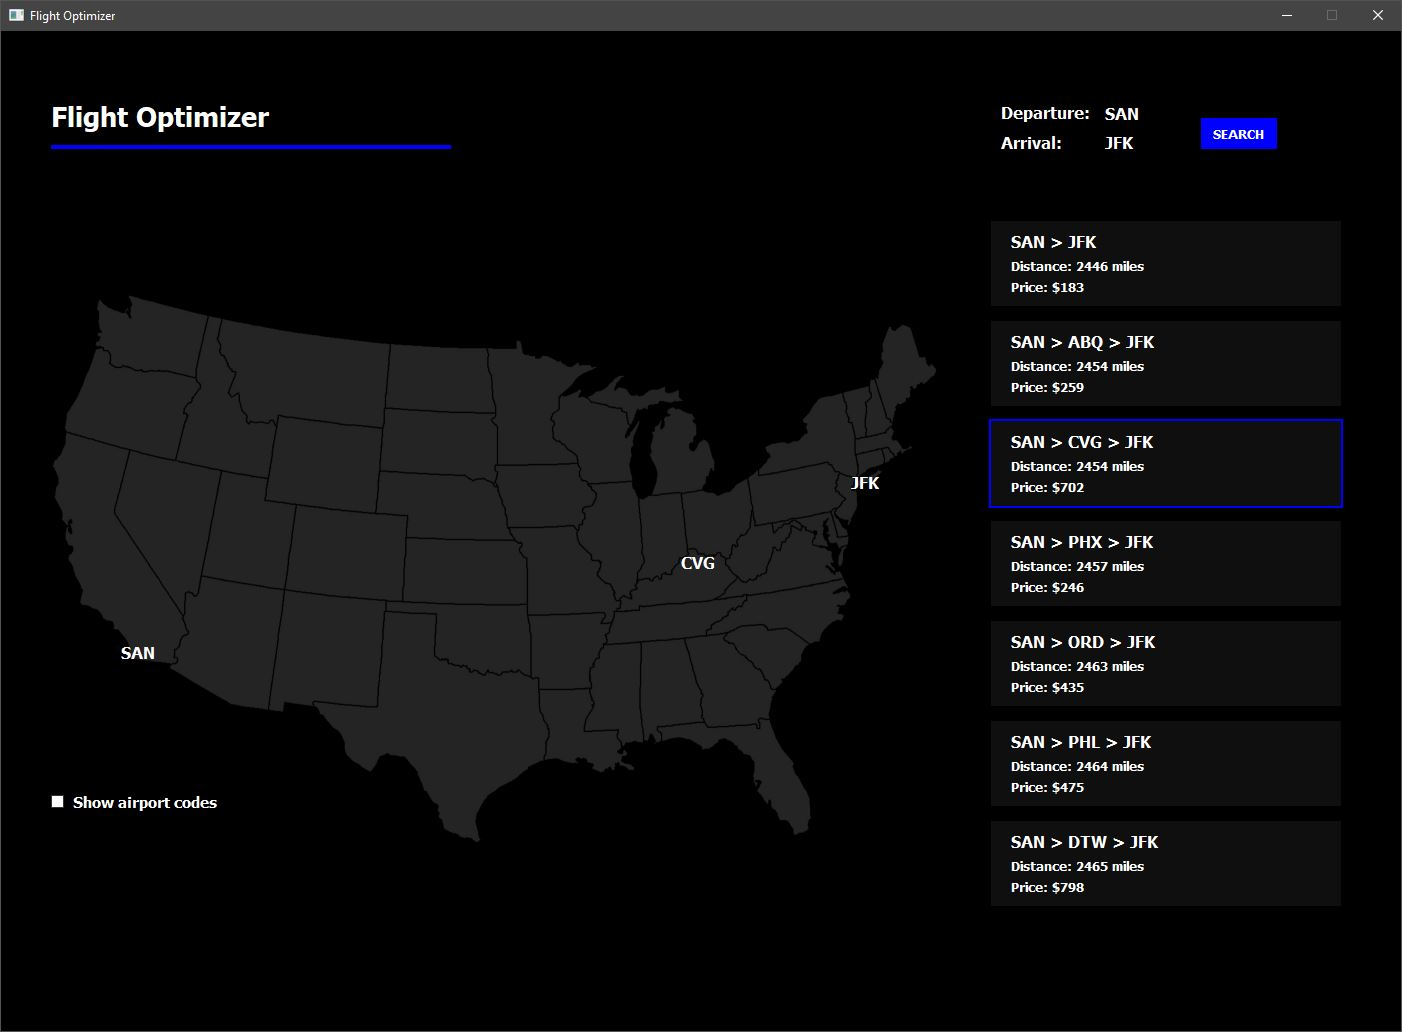
\includegraphics[width=0.9\textwidth]{app.jpg}
\end{SCfigure} \\


\section*{Research Question}

\noindent
How can optimal flight paths between two airports in the United States be computed?

\section*{Introduction}

\noindent
November last year, I was searching flights to go from Madrid (Spain) to Toronto. I simply went to “Google Flights” and marked Madrid as the departure city and Toronto as the destination. The site gave me a list of over 20 possible flight combinations I could take. The first combination was to fly to Lisbon (Portugal) and from there fly directly to Toronto. I believe this combination appeared the first one because it was the cheapest and the quickest. Another option was to travel to London (UK) and then go to Toronto. I remember this option took a bit longer and it was around 50€ more expensive. This is why I ended up choosing the first option. \\

\noindent
Now that we have studied data structures such as Graphs, I can get a sense of how flight websites go about finding optimal combinations to get to a desired destination. Conceptually, a flight network could be graph where the nodes are the airports, and the edges are the flights connecting these airports. To get all the possible flight combinations to go from airport A to airport B, we would need to traverse the graph, node after node, starting at A and finishing at B. Since airports usually have many incoming and outcoming connections, the number of possible paths from A to B can get very large, especially when considering the whole world as the flight network! There are certainly flight combinations that start in Madrid, go all the way to Singapore, make a layover in Moscow and end up Toronto. This of course, would be an extremely long and expensive journey. The goal in this project is to find a way to avoid exactly this type of inefficient flight combinations and compute the most efficient path. To make the study more focused, I decided to limit myself to national flights within the United States.


\section*{Dataset}

\noindent
For this project I used a dataset created by Ryan Zernach (2018 Airplane Flights) which includes over 1 million flights from airports all round the US. The data corresponds to predictions based on a statistical analysis of real flight data. The original data has the following format:\\

\begin{SCfigure}
    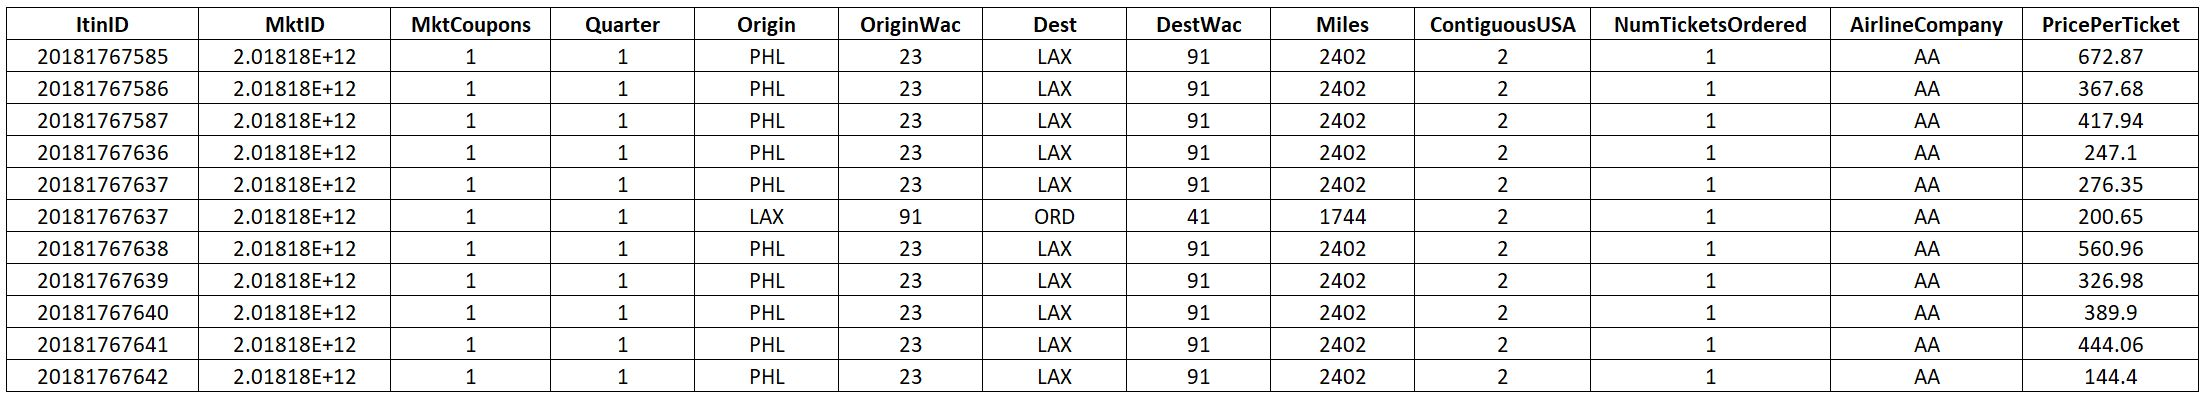
\includegraphics[width=0.9\textwidth]{table1.jpg}
\end{SCfigure} \\

\noindent
In the program I am only interested in the origin (departure) airport, the destination airport, the distance of the flight (in miles), the price per ticket and the airline company. This is why I modified the original csv file to only include these columns.\\

\begin{SCfigure}
    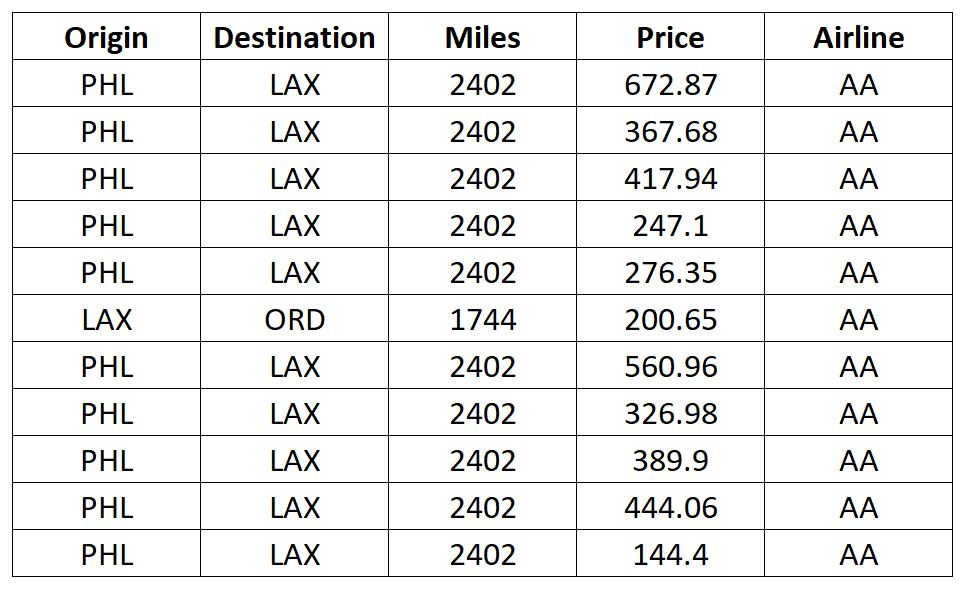
\includegraphics[width=0.35\textwidth]{table2.jpg}
\end{SCfigure} \\

\noindent
With this dataset, I have access to variety of flights across the US and I can use it to build a model of a Flight Network which can be represented as a graph. Note that each line in the csv file represents a single flight which represents an edge in the graph. The origin and destination airports represent vertices in the graph.\\

\section*{Computational Overview}\\

\noindent
The program allows the user to specify a departure airport and a destination airport. After pressing the “SEARCH” button a list of possible flight combinations appears and the path of the selected combination is shown on a map of the US (the code of each airport in the path appears at its corresponding geographical location).\\

\noindent
\underline{Flight Network class}\\

\noindent
To accomplish this functionality, I started by creating a FlightNetwork class which is a variant of class representing a graph. The class implements this graph behavior with a private variable called \_flights which stores a dictionary with keys representing airports and the values representing a set of outgoing direct flights from an airport. Airport and Flight are two other created classes.\\

\noindent
\_flights has the following format:\\

\noindent
\{\\
\indent
Airport: \{ Flight, Flight, Flight, … \},\\
\indent
Airport: \{ Flight, Flight, Flight, … \},\\
\indent
Airport: \{ Flight, Flight, Flight, … \},\\
\indent
…\\
\}\\

\noindent
With the FlightNetwork class, we can perform all kinds of graph computations that will allow us to find optimal flight paths between two airports (which is the end goal of this project).\\

\noindent
\underline{Loading the graph}\\

\noindent
The first step in the program is to load this network using the csv file described in the previous section. I abstracted this functionally into a method of FlightNetwork simply called load which takes in a str parameter for the file path of the dataset. Using the csv reader in Python, I managed to loop through each line in the file and store the data in an array of str called row.\\

\noindent
To create the departure and destination Airport classes I used row[0] and and row[1].\\

\noindent
departure = Airport( row[0], “” )\\
destination = Airport( row[1], “” )\\

\noindent
(The second argument corresponds to the city of the airport. It is left as an empty string but this can be improved in future versions of the program.)\\

\noindent
To the create Flight class, I used departure, destination, row[2], row[3] and row[4].\\

\noindent
flight = Flight( departure, destination, int(row[2]), float(row[3]), row[4] )\\

\noindent
Having a departure Airport class and a Flight class for each line in the csv file, we can now add a new entry to the \_flights dictionary.\\

\noindent
self.\_flights[departure].add( flight )\\

\noindent
\underline{Computing paths between two airports}\\

\noindent
Once the graph is loaded, we can compute the possible paths between two vertices. I defined a public method get\_paths to find the possibles paths in the Flight Network and a private method \_get\_paths\_recursion which serves a helper method for get\_paths to perform recursion.\\

\begin{SCfigure}
    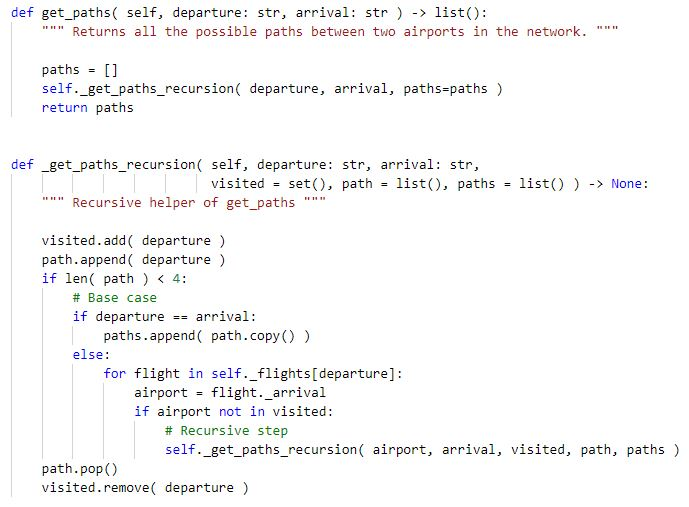
\includegraphics[width=0.7\textwidth]{code1.jpg}
\end{SCfigure} \\

\noindent
The base case occurs when departure == destination. When this statement is true we have found a valid path through the network and we can append it to the paths list. When the statement is false, we loop trough all the outgoing flights from departure, use the destination airport as the departure, check that it wasn’t visited already, and perform recursion passing a reference of the current path (which gets the new airport appended at the beginning of the \_get\_paths\_recursion method).\\

\noindent
\underline{GUI}\\

\noindent
The Graphical User Interface is a very important part of the program since it allows the user to visualize the results of the computations taking place in the background. To create this GUI, I used the library pyqt5 which comes with many features that ease the development of this interface. I created a module called gui.py which is responsible for all the QT specific code. In there, I created a set of functions that abstract the QT API calls and which can be used in other modules, particularly in main.py. For example, the contents of on\_app\_start in main.py, are executed when the QT application starts. Another example is set\_departure\_text which directly modifies the GUI at runtime at sets the text of the element displaying the code of the departure airport.\\

\noindent
In gui.py I also placed automatically generated code from QT which defines the layout of the GUI. To get this code I used the program QT designer, where I was able to drag and drop GUI elements and create the layout of the app.\\

\noindent
\underline{Logic behind “SEARCH”}\\

\noindent
After specifying the departure and destination airports codes the user can press the search button to get the results of the query. The list of possible flight paths appears below the button and the selected path is shown on the map.\\

\noindent
Firstly, we need to get all the possible paths using the values in the departure and destination text fields. We can use gui.get\_departure() and gui.get\_destination() to get these values and then network.get\_paths( departure, destination ) to get the paths.\\

\noindent
To display the path visually in the list items we need to extract the a text of the form “SAN $>$ LAS $>$ SFO”, the total distance and the total price. For this, we need to loop through each path in the all the possible paths and then inside that loop, loop through each airport in the path. We can use network.get\_connecting\_flight( path[i], path[i+1] ), where i is the loop variable of the inner loop, to ge the connecting Flight class and extract the distance and price (we can get the total distance/price by adding each of the values from each flight together).\\

\begin{SCfigure}
    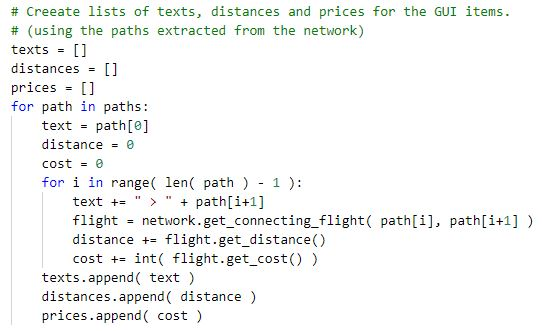
\includegraphics[width=0.6\textwidth]{code2.jpg}
\end{SCfigure} \\

\noindent
We can then sort texts, distances and prices and display each index of the lists in the corresponding GUI item using gui.set\_flight\_path\_text, gui.set\_flight\_path\_distance and gui.set\_flight\_path\_price. Currently, the program sorts the item based on the total distance. This could be improved using a combination of distance and price or use user defined filters (see Discussion for more details).\\


\section*{Instructions for running the program}

\noindent
1.	Install pyqt5\\
2.	Extract the content of dataset.zip (it should contain a file called “flights.csv”).\\
The zip file was placed in the MarkUs submission and can also be found here:\\
https://utoronto-my.sharepoint.com/:u:/g/personal/juan\_martin\_mail\_utoronto\_ca/EaU8xtePRNBOn2kJLwfPgv4B-kIrBj-CSYjnPYrPJCeSBA?e=6HGtX2\\
3.	Create a new folder.\\
4.	Place main.py, flight\_network.py, gui.py and flights.csv in the new folder.\\
5.	Double-click main.py\\
6.	A console will appear and the data from the csv file will start to be loaded into the app.\\
7.	When the data is loaded, the GUI will appear and should look like the image at the beginning of this document.\\

\noindent
The user will be able to type airport codes, search flight paths and visualize in a list of items below the search button and the airport codes of the selected path should appear on the map. When pressing on any of the list items, the widget should be bordered in blue and the corresponding path should appear on the map.


\section*{Changes post proposal}

\noindent
The general idea form the proposal was kept; a program to visualize flight paths between two airports in the US. Nonetheless, to compute these paths I ended up nor using Dijkstra’s algorithm or any variant such as A*. Doing more research into those topics I found out that these algorithms are great for finding the best unique path but since I am interested in finding multiple possible paths, I ended up using a recursive pattern (similar to the one studied in class) and limit the length of the paths to a maximum of 3 airports to reduce the computational time (which turned out to be great, the results appear immediately after pressing “search”).

\section*{Discussion}

\noindent
Our initial motivation was: How can optimal flight paths between two airports in the United States be computed? Even though there many systems and algorithms coming together to create the app, the core of the program lies in the recursive pattern of the get\_paths method. Recursion allowed to very efficiently traverse the graph and find possible paths going neighboring airport after neighboring airport.
Reducing the maximum length of the path to 3 makes the algorithm very fast because the program won’t need to recurse into every single possible path. This program could be applied to larger network (such as the whole world) and the computational time would be pretty much the same. Also, having more than 3 airports in the path is not very practical and it very uncommon to take that many stops in a travel (if we were using the whole world, we could increase this number to 4 or even 5 for very remote destinations).\\

\noindent
The main limitation of the program is that we are a using a fixed dataset of flights and not real time flights. Some flights appear several times in the file with different prices but he same departure and destination. In the code, I selected the flight that appear the first and added to the graph. Using this dataset, I could get all the flights with the same departure and destination and add the average price to the graph. This would give more accurate prices but would still not be useful for real clients (the flights are not real-time). 
Using a library like scrapy would help solving this problem since the dataset would be loaded and updated with flights found by scraping the web.\\
Another limitation coming from the dataset used is that the loading time at the beginning of the program is quite significant. In my computer it takes around a minute to load all the data. If we were to use a larger dataset with more airports and connecting flights, the loading time would increase accordingly. Using scrapy would also solve this problem since the app would not have to load all the data every time the app starts. Perhaps the model could be loaded in a server independent to the client’s computer and a web scraper would look for new flights at constant intervals during the day and update the model accordingly. The client would then send a request to the server (without having the model stored locally) and the server would use its model to send the list of flights.\\

\noindent
Here are some other ideas for future development:\\

\noindent
• Use user defined filters for the list of flight paths (total distance, total cost, airline, date).\\
• More path results in the form of a scrollable list. Currently, the app has 7 fixed items for displaying flight data.\\
• Show connecting airports with a line. This would be a lot more aesthetic and easier to visualize where the plane will go through. Another neat addition would be to add an animation of a small 2d plane travelling through the path.\\
• The airports codes added to the map are not all the airports in the US and not even all the airports in the dataset. Adding more to map would make the app more robust and complete. Currently when an airport is not in the GUI a warning message appears in the console and the path is not displayed on the map.\\
• Expand the network to international flights outside the US. For this I would be adding the airport codes manually to the GUI and would need to implement an algorithm that would do it automatically. This could be achieved using a different dataset with airports and their world coordinates.\\
• Make the project web application. For the purpose of finding flight paths, I think a web app is much more useful for the end user. I could use a framework such as Django that utilizes Python and port the code from this project.


\section*{References}

\noindent
“A* (A Star) Search Algorithm - Computerphile.” Performance by Mike Pound, YouTube, Computerphile, 15 Feb. 2017, www.youtube.com/watch?v=ySN5Wnu88nE&amp;t=27s.\\

\noindent
“Dijkstra's Algorithm - Computerphile.” Performance by Mike Pound, YouTube, Computerphile, 4 Jan. 2017, www.youtube.com/watch?v=GazC3A4OQTE.\\

\noindent
“A Fast and Powerful Scraping and Web Crawling Framework.” Scrapy, scrapy.org/.\\

\noindent
“Getting Started with PyQt.” PyQt/Tutorials - Python Wiki, wiki.python.org/moin/PyQt/Tutorials.\\

\noindent
JaapVanDerAar. “JaapVanDerAar/Flight-Network-Analysis.” GitHub, github.com/JaapVanDerAar/Flight-Network-Analysis.\\

\noindent
Joshi, Vaidehi. “Finding The Shortest Path, With A Little Help From Dijkstra.” Medium, Basecs, 17 Oct. 2017, medium.com/basecs/finding-the-shortest-path-with-a-little-help-from-dijkstra-613149fbdc8e.\\

\noindent
“PyQt5.” PyPI, pypi.org/project/PyQt5/.\\

\noindent
Zernach, Ryan. “2018 Airplane Flights.” Kaggle, 16 Nov. 2019, www.kaggle.com/zernach/2018-airplane-flights.\\


\end{document}